\documentclass[journal]{IEEEtran}
% *** CITATION PACKAGES ***
\usepackage{url}
\usepackage{cite}
\usepackage{graphicx}
\usepackage{amsmath}
\usepackage{dblfloatfix}
\usepackage{threeparttable}
\interdisplaylinepenalty=2500
\usepackage{array}
\usepackage{multirow}
\usepackage{lipsum}% http://ctan.org/pkg/lipsum
\ifCLASSOPTIONcompsoc
\usepackage[caption=false,font=normalsize,labelfont=sf,textfont=sf]{subfig}
\else
\usepackage[caption=false,font=footnotesize]{subfig}
\fi
\ifCLASSOPTIONcaptionsoff
\usepackage[nomarkers]{endfloat}
\let\MYoriglatexcaption\caption
\renewcommand{\caption}[2][\relax]{\MYoriglatexcaption[#2]{#2}}
% lipsum allows figs/tables to cross-double rows. 
\fi


\begin{document}
	% Do not put math or special symbols in the title.
	\title{Characterization of the Neutron Energy Spectrum of the AFIT Graphite Pile and NIF Experiment}
	
	\author{Nicholas~Quartemont}
	
	% The paper headers
	\markboth{Characterization of the Neutron Energy Spectrum of the AFIT Graphite Pile and NIF Experiment}%
	% A title should better capture what the article is about to draw readers in.  This to me sounds like a review article, which this is not
	{Shell \MakeLowercase{\textit{et al.}}: Characterization of the Neutron Energy Spectrum of the AFIT Graphite Pile and NIF Experiment }

	% make the title area
	\maketitle
	
	% This first commit show a technique that makes it easier to edit and see the edits.  If each sentence is it's own line, then the diff between the files will only show lines that changed.  Otherwise, you have to find the change, which may be small, in a para of text.
	\begin{abstract}
		\ This paper outlines a foil activation experiment performed at the Air Force Institute of Technology neutron pile.
The purpose of the experiment was to measure the neutron flux spectrum in stringer 2 using foil activation unfolding techniques such as STAYSL. 
Due to facility limitations, the unfolding analysis was conducted on an experiment with a test snout performed at the National Ignition Facility (NIF). 
Foil activation experiments are an indirect method of measuring an incident neutron flux and are preferred in high flux environments that will damage electronics or for size constraints. Foil activities produced from threshold and non-threshold reactions were analyzed using a high purity germanium detector that resulted in time-corrected activities post-irradiation in the range of 100 Bq to 10 kBq. The NIF experiment utilized aluminum, gold, indium, and zirconium foils of varying mass at the pinhole, basket, and kinematic base locations of the snout. The irradiation planned for the neutron pile also included tungsten and manganese. The incident neutron fluence was unfolded from the activities and nuclear data with a simulated NIF guess spectrum through iterative execution of STAYSL. The iteration was completed with and without updating the uncertainty from STAYSL at each step. The results for the pinhole and basket show varying results that did not agree well with the modeled result. The pinhole without the uncertainty updated provided spectrum that was not rejected; however, the results for the basket do not match intuition or the model. The result for the kinematic base resulted in a spectrum that is consistent with the model, nuclear data, and foil activations in both cases. Three potential reasons for the discrepancies include the foil material parameters, modeled spectra, and uncertainty in the NIF source. 

	\end{abstract}
	
	% Note that keywords are not normally used for peerreview papers.
	\begin{IEEEkeywords}
		neutron flux unfolding, foil activation, high purity germanium, STAYSL 
	\end{IEEEkeywords}
	
	\IEEEpeerreviewmaketitle
	
\section{Introduction}
\IEEEPARstart{C}{characterizing} an energy dependent neutron environment has many applications to the nuclear sciences community. Determining a neutron flux is important for experiments where the neutron flux requires validation or is not well modeled. Neutrons can be detected using a variety of methods, such as Bonner spheres, time of flight spectroscopy, long counters, He-3 based detectors, or proton recoil scintillators \cite{Knoll}. Foil activation experiments can also be performed to acquire an indirect measurement of the incident neutron fluence on a set of activation foils. Activation experiments are essential for testing that requires small geometry to fit in the apparatus or in situations where electronics equipment for higher fidelity measuring techniques will be damaged. 

\ This work aims to outline an experiment to characterize the neutron spectrum in the Air Force Institute of Technology's (AFIT) Building 470 neutron pile constructed in the 1960s which contains a plutonium-beryllium (PuBe) neutron source \cite{NETF}. Previous studies accomplished results indicating changes to the neutron source term and modeled the neutron flux at various positions \cite{Bevins,Will}. However, the pile spectrum was not fully experimentally characterized. A neutron source characterization was performed with a foil activation experiment. The foils were intended to be analyzed using a calibrated high purity germanium (HPGe) detector to determine time corrected activities post-irradiation. The HPGe was calibrated for energy and efficiency to back out the initial foil activities post-irradiation. 

\ The pile activation results were not used in the final neutron flux unfolding due to issues with the HPGe at AFIT. Instead, this work analyzed an experimental setup at the National Ignition Facility (NIF). The NIF foil activation experiment was performed on a snout for a shot performed in March 2018\cite{Bogetic}. The goal of the NIF experiment was to characterize the NIF source in the aluminum snout which has applications for exploring cross-section uncertainties if there are unexpected results. The incident neutron flux was unfolded from the foil activation results using Pacific Northwest National Laboratory (PNNL) STAYSL which uses generalized least-square minimization to determine the flux spectrum for given foil activities and nuclear data\cite{STAYSL}.

\ This paper describes the problem description for the foil activation experiment at the AFIT pile and NIF. Relevant theory is presented including foil activation, HPGe, and neutron flux unfolding. Additionally, the work performed outlines the foil selection process, HPGe characterization, and NIF modeling. Finally, the results of the unfolded NIF spectra are presented. 

\section{Problem Description}.
\ Unfolding a neutron flux from the nuclear data and foil activations is dependent on the source, modeling, activation foils selection, and foil activations produced. The process for solving the unfolding problem was carried through the HPGe characterization for the AFIT neutron pile experiment. The remaining portions of the process, HPGe results and STAYSL, were aimed at the NIF experiment. The following sections summarize the main problem contributions for each experiment.  Supporting documentation and work performed is available on Github\cite{Me}. 

\subsection{Building 470 Pile Neutron Environment }
\ Previous work completed a rough model of the AFIT pile and studied the energy dependent neutron flux as a function off position in the pile and stringers\cite{Will}. The neutron pile was modeled in MCNP version 6.1 
based on the previous work to gauge expected flux distributions\cite{MCNP}. Stringer 2 was determined to have the highest level of neutron flux which is expected from its close proximity to the PuBe source. The setup of foil placement and PuBe source is shown in Figure \ref{fig:pile}. The pile stringers contain fabricated placements for the source and foils to help ensure repeatability of measurements. 

\begin{figure}[h!]
	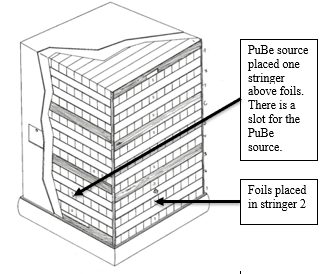
\includegraphics[width=\linewidth]{Figures/PileSetup.png}
	\caption{Activation foil setup for Building 470 graphite pile irradiation.}
	\label{fig:pile}
\end{figure}

\ The starting PuBe neutron spectrum, shown in Figure \ref{fig:PuBE}, has a maximum energy of approximately 11 MeV and peaks near 3.5 MeV. 
However, there is significant thermalization of the starting PuBe spectrum by the graphite pile as shown in the simulated stringer 2 spectrum in Figure \ref{fig:Spec1}. 
The simulated spectrum was used to select activation foils based on the modeled foil activation rates, discussed in Section 3. 

\begin{figure}[h!]
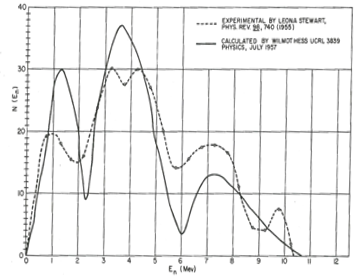
\includegraphics[width=\linewidth]{Figures/PuBe.png}
\caption{PuBe neutron emission source spectrum.}
\label{fig:PuBE}

\vskip 0.25cm

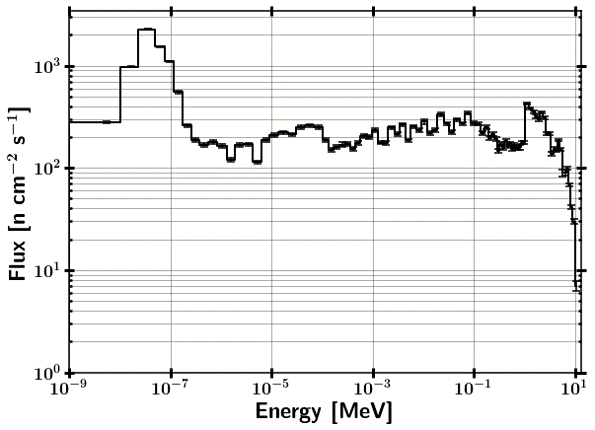
\includegraphics[width=\linewidth]{Figures/PileSpec.png}
\caption{Foil activation neutron flux spectrum (all statistical errors are under 1.5 percent).}
\label{fig:Spec1}
\end{figure}


\subsection{NIF Snout Experiment}

\ The passive foil activation experiment was performed in 2018 at the NIF. A snout composed of aluminum was mounted to the Target and Diagnostic Manipulator (TANDM) 90-348. Three foil activation diagnostic packs of aluminum, zirconium, indium, and gold were placed in the nose cap pinhole (7 cm from source), filter basket (41 cm), and kinematic base (110 cm). The aluminum foil was not used in the pinhole. Figure \ref{fig:NIF} displays the snout with the activation foil sites \cite{Bogetic}. 

\begin{figure}[h!]
	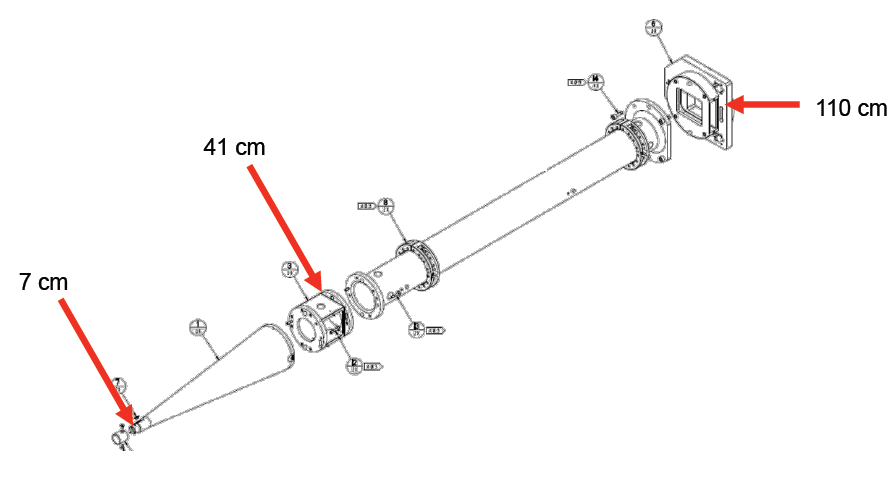
\includegraphics[width=\linewidth]{Figures/NIF.png}
	\caption{Passive NIF snout foil activation locations.  Foils were placed in the nose cap pinhole (7 cm), filter basket (41 cm), and kinematic base (110 cm).}
	\label{fig:NIF}
\end{figure}

\ The NIF source was a D-T Polar Drive Exploding Pusher (PDXP) target with a nominal yield of  $3.7*10^{15}$ neutrons \cite{NIFSrc}. The neutrons were at a mean energy of 14.06 MeV and a theoretical thermal plasma temperature of 10.75 keV which creates a spread in the neutron energies. The resultant Gaussian distribution centered at 14.06 MeV has a full width at half maximum of approximately 0.8 MeV\cite{Appelbe}. The unnormalized source probability distribution function is shown in Figure \ref{fig:NIFSRC}. The spectrum of neutrons was used as a source term for an MCNP simulation to determine the guess foil neutron spectrum in Section 3. 

\begin{figure}[h!]
	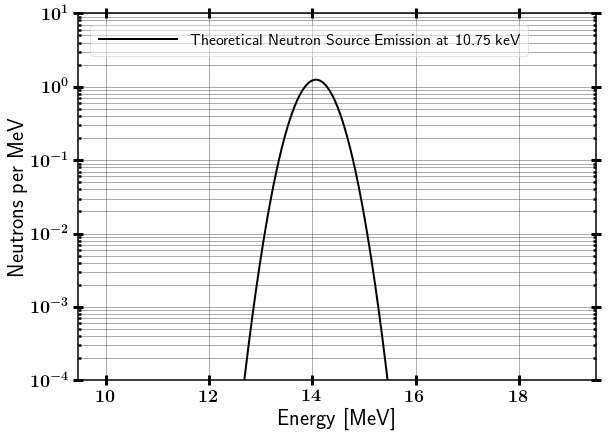
\includegraphics[width=\linewidth]{Figures/Applebe1075keV.png}
	\caption{10.75 keV D-T fusion source distribution.}
	\label{fig:NIFSRC}
\end{figure}

\section{Description of Work}
	\begin{table*}[!b]
		%	\begin{threeparttable}[!b]
		
		\caption{Activation foils selected for irradiation in neutron pile.}
		\label{tab:foils1}
		%		\width=17.5cm
		\centering
		\begin{tabular}{|c|c|c|c|c|c|c|}
			\hline
			Foil (thickness) & Reaction & Half-life & \begin{tabular}[c]{@{}c@{}}Threshold\\   {[}MeV{]}\end{tabular} & \begin{tabular}[c]{@{}c@{}}Decay\\   Radiation {[}keV{]} \\ (Intensity)\end{tabular} & Elemental Purity {[}\%{]} & Mass {[}g{]} \\ \hline
			\multirow{2}{*}{In (0.005'' x2)} & In-115 (n,g) In-115m & 54.29 min & Thermal & 1293.56 (0.848) & 99.99 & 0.2217 \\ \cline{2-7} 
			& In-115 (n,n') In-116m & 4.49 hrs & 0.336 & 336.24 (0.459) & 99.99 & 0.2217 \\ \hline
			Al ($\sim$2mm x4) & Al-27 (n,a) Na-24 & 15.00 hrs & 3.25 & 1368.63 (0.9999) & $99^{\dag}$ & 3.3953 \\ \hline
			\multirow{2}{*}{Au (0.005'' x2)} & Au-197 (n,2n) Au-196 & 6.17 days & 8.11 & 355.7 (0.87) & 99$^{\dag}$ & 0.5772 \\ \cline{2-7} 
			& Au-197 (n,g) Au-196 & 2.69 days & Thermal & 411.8 (0.9562) & $99^{\dag} $& 0.5772 \\ \hline
			W (0.005'' x2) & W-186 (n,g) W-187 & 24.00 hrs & Thermal & 685.51 (0.332) & 99.98 & 0.6272 \\ \hline
			\begin{tabular}[c]{@{}c@{}}Mn (0.068 mm \\ to 0.077 mm) x4\end{tabular} & Mn-55 (n,g) Mn-56 & 2.58 hrs & Thermal & 846.8 (0.9885) & $99^{\dag}$ & 0.2660 \\ \hline
			\begin{tabular}[c]{@{}c@{}}Zr (Not used in\\  Pile Experiment)\end{tabular} & Zr-90 (n,2n) Zr-89 & 78.41 hrs & 12.1 & 909.2 (0.9904) & N/A & N/A \\ \hline
		\end{tabular}
		\begin{tablenotes}
			\item[\textdagger] $\qquad \quad$  \textdagger $\quad $ The 99\% elemental purities are assumed
		\end{tablenotes}
		%		\end{threeparttable}
	\end{table*}
	
	\subsection{AFIT Pile Activation Foils and Irradiation Parameters}
	% This section feelsmore relevant to a lab report or thesis.  For a journal article, you can reference sources for foil constraints and highlight whichever affected you selection process.  You can then show the equuations you used to get the time zero activities, and the corrections applied, from the counts.  For example, you didn't explicitly do a backgroud count to subtract, this was done via fitting, so the equation and description don't match what was done and is more academic in nature.
	
	\ The selected foils for the experiment are summarized in Table \ref{tab:foils1}. 
	The foils were selected based on availability, the nuclear data libraries used by STAYSL, reaction cross-section, decay mechanism, and saturation activations. Desirable characteristics of activation foils have been well established in literature \cite{Knoll,Luciano2012a,Kuijpers1977}.
	
	\ The International Atomic Energy Agency provides data for the IRDFF library which contains benchmarked neutron dosimetry reactions\cite{Greenwood2016}. This library is used in the PNNL STAYSL code system, and all of the reactions used for this foil activation experiment have nuclear data within the IRDFF. The IRDFF v1.05 library contains ``state-of-the-art" covariance information and has continuous improvement through testing and integral experiments \cite{Greenwood2016}. 
	
	\ The cross-section was considered for two main reasons. First the uniqueness of the cross-section shape was used to unfold the incident neutron energy spectrum. An (n,$\gamma$) cross-section may peak in a particular region, which is essential to providing information of the neutron flux in that energy region. Alternatively, a threshold reaction, 
	such as an (n,2n), is important for providing information of the flux at higher energies. Additionally, the selected foils were chosen to cover the entire energy range of the incident neutron flux. The threshold energy for each reaction is noted in Table \ref{tab:foils1}.
	
	\ Foil activation production rate of radioactive isotopes is negated by radioactive decay processes, which place an upper limit on the radioactivity of a foil \cite{Knoll}. The saturated activity, ($A_{\infty}$), for a given reaction is given by, 

	\begin{equation} \label{eq:InfReactionRate}
	A_{\infty} = R = \int_{E1}^{E2} \phi(E) \Sigma(E)_{act} V
	\:dE ,
	\end{equation}
	
	\noindent where the saturated activity is equivalent to the reaction rate (R), which is a function of the energy dependent flux ($\phi$), the macroscopic reaction cross-section for the activation reaction channel ($\Sigma(E)_{act}$), and the volume of the foil ($V$). The energy term ($E1$) is zero in reactions with no energy barrier; however, threshold reactions require the incident neutron to be of higher energy to enable the reaction channel. 
	
	\ The foils were modeled in MCNP to produce a reaction rate for the pile neutron flux environment which was used to determine the irradiation time with the saturation activity taken into consideration. The MCNP result indicates no feasible reactions in the high energy region, such as the (n,2n) threshold reactions. The lack of pinning at high energy is potential issue for the neutron flux unfolding where there is no reaction pinning the high end of the neutron energy spectrum. A correction was included to account for saturation in the foil. The activation of the foil for a given	irradiation time ($t_{i})$ is given as a function of the decay 
	constant: 
	
	\begin{equation} \label{eq:ReactionRate}
	A_{0} = A_{\infty}(1-e^{-\lambda t_{i}}) 
	\end{equation}
	
	\ The irradiation time in the neutron pile was planned to be ten days. This time was chosen to build up the enough activity to be able to count the foils to approximatley 1\% counting statistics. At six half-lives a foil will have reached approximately 98\% of its saturation activity, neglecting spatial and energy self-shielding effects \cite{Knoll}. Ten days is over six half-lives for most of the activation products. The expected post-irradiation activities is summarized in Table \ref{table:active}.  
	
	\begin{table}[h!]
		\caption{Activation information for selected pile foils.}
		\label{table:active}
		\centering
		\begin{tabular}{|c|c|c|c|}
			\hline
			Reaction & \begin{tabular}[c]{@{}c@{}}A\_\{inf\}\\ {[}Bq{]}\end{tabular} & \begin{tabular}[c]{@{}c@{}}A\_\{0\}\\ {[}Bq{]}\end{tabular} & \begin{tabular}[c]{@{}c@{}}Count Time to \\ 10,000 Counts \\ (at 1\% efficienty)\\ {[}hrs{]}\end{tabular} \\ \hline
			W-186 (n,g) W-187 & 177 & 176 & 9 \\ \hline
			In-115 (n,g) In-115m & 1394 & 1394 & 1 \\ \hline
			Au-197 (n,g) Au-196 & 820 & 685 & 7 \\ \hline
			Mn-55 (n,g) Mn-56 & 256 & 256 & 3 \\ \hline
			All others & \textless 1.0 & \textless 1.0 & N/A \\ \hline
		\end{tabular}
	\end{table}
	
	\ The production rate formula was simplified in the limit of irradiation times much less that the half-life of the activation products. In this case, the reaction rate is much larger than the decay from radiation, so the rate of production of the radioisotope is driven primarily by the reaction rate. The time integrated flux, or neutron fluence ($\Phi$), can be used to determine the total reactions, $R_{total}$, over an irradiation period. If the temporal aspect of the neutron flux is very short, such as at the NIF, the interpretation of the flux given by STAYSL can be interpreted as a fluence by:
	
	\begin{equation} \label{eq:NIFrxnRate}
	R_{total} = \int_{E1}^{E2} \Phi(E) \Sigma(E) _{act} V 
	\:dE 
	\end{equation}
	% Is Eq 4 used anywhere? Not specically, it just shows why the NIF results are a fluence. 

	\ Another consideration for the foil selection process was the decay constant of the product nuclides. The half-lives applicable for a particular experiment depend on the time post-irradiation that the foils can be counted. A long lived radioisotope will be available for counting for longer times, but the activity will be reduced due to the lower decay constant. The opposite is true for short	half-lives. A half-life on the order of an hour to a few years is in the right direction; however, the half-life must also be balanced with the production of the radioisotope to understand the entire picture. 
	
	Additional information was taken into account for the activation foil selection. First, foils with interfering reaction channels and decay emissions were avoided. Second, the activation foils needed to be optically thin so as to not cause perturbations of the neutron flux. An additional benefit of relatively thin foils was that the gamma-ray emissions are not significantly attenuated through self-shielding. Finally, only gamma-ray emitter radioactive products were considered. Gamma-ray detection can provide fine energy resolution to determine activation due to specific reaction channels. Beta spectroscopy was not considered; however, it is a potential option. 
	
\subsection{HPGe Calibration}

\ An ORTEC HPGe was connected to a DSA1000 which functions to replace many components necessary for a traditional nuclear detection system. The DSA1000 was connected to a computer using the Genie 2000 multi-channel analyzer (MCA) data acquisition software. The bias voltage is set to -4,000 V. The gain was set to 20 and the fine gain to 1.5, this allowed the dynamic range of the MCA to cover the gamma ray energies of interest. 

%It was negative, right? It depends which one we were using. 

\ The HPGe was characterized using a multi-nuclide source. The isotopes gamma decay energies in the source range from 60 keV from Am-241 to 1836 keV from Y-88, which covers the energy range of interest for the foil analysis. An energy calibration using a linear relationship to map energy to channel resulted in 0.2583 keV per channel with an offset of 0.0413 keV. 

\ The efficiency calibration spectrum was captured at 10 cm and 5 cm from the base of the HPGe. An malfunction in the HPGe occurred prior to the completion of collecting data for the 5 cm case. The error prevented additional data acquisition for the building 470 pile portion of this experiment. The absolute efficiency was to be calibrated at a source distance to obtain the unknown source activity from the activation foils \cite{Knoll}. The absolute efficiency ($\epsilon_{abs}$) is given by:

\begin{equation} \label{eq:effa}
\epsilon_{abs} =\frac{\text{\# Events Recorded}}{\text{\# Radiation Quanta Emitted}}
\end{equation}

\ A calibrated efficiency curve was planned to be used to find the source strength of samples, scaled by the distance to the detector. There are a few types of fits that are appropriate for efficiency curves. A common efficiency curve given as a function of N fitting parameters and a reference energy ($E_{0}$) to be used in this work was:
%Piece-wise curves can work in certain applications, where a . % which ones? I was going to say something, but I think it is just a lazy fit now. 

\begin{equation} \label{eq:effa1}
	ln(\epsilon_{abs}) =   \sum_{i=1}^{N} \; a_{i} (ln(\dfrac{E_{\gamma}}{E_{0}}))^{i-1}
\end{equation}

Experimental measurements also need to be corrected to deduce the original activity of the foil post-irradiation. The measured counts of the HPGe full energy peak, $C$, was determined from the activation foil spectroscopy. The activity is corrected for the radioactive decay for the time between the end of irradiation and the start of counting ($t_{d}$). A similar correction factor based on the count time, $t_{c}$ provided a correction for radioactive decay during counting. Additionally, the detector efficiency for the given gamma-ray energy, $\epsilon$, and relative gamma intensity, $I_{\gamma}$, must be taken into account. The gamma intensity may also include a branching ratio if applicable to the decay mechanism. All corrections included, less self-shielding effects, provide a formulation for converting counts to post-irradiation activity as: 

\begin{equation} \label{eq:MeasActivity}
A_{0} = \frac{\lambda (C) e^{\lambda t_{d}}}{\epsilon (1-e^{-\lambda t_{c}})I_{\gamma}}
\end{equation}

\subsection{NIF HPGe Spectroscopy}

\ The HPGe analyzed dataset used for the NIF experiment was provided from Lawrence Livermore National Lab (LLNL). The counts per channel data were also provided. A validation test was performed with Los Alamos National Laboratory's Peak Easy on the pinhole results for the indium foil\cite{PeakEZ}. The main In-115m peak at 336 keV is shown in Figure \ref{fig:peakez}. This fit was performed with a step function using cubic interpolation of the background with a low energy tail. 

\begin{figure}[h]
	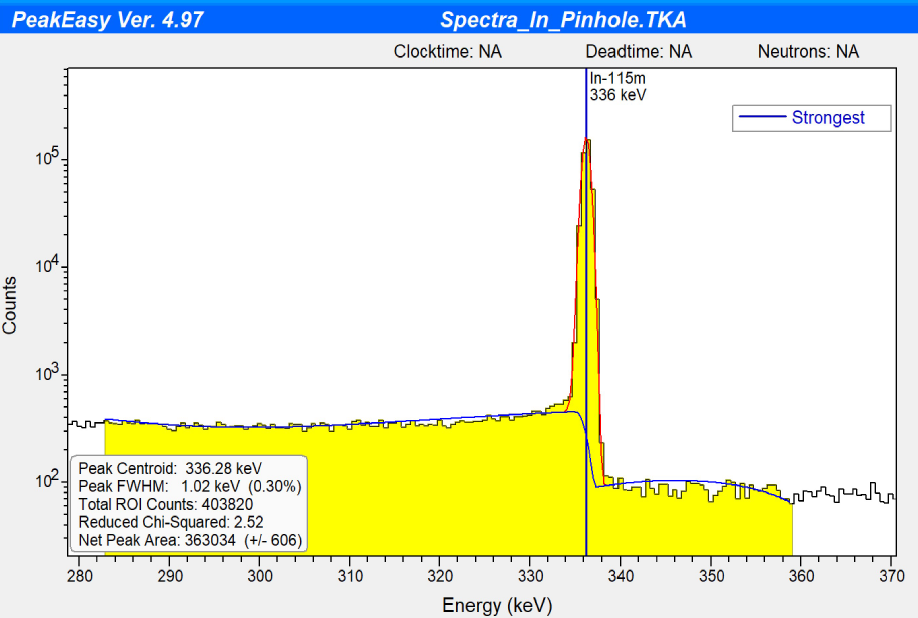
\includegraphics[width=\linewidth]{Figures/PeakEZ.png}
	\caption{336 keV In-115m peak counts determined using Peak Easy Version 4.97.}
	\label{fig:peakez}
\end{figure}

% The background subtraction looks terrible.  It probably doesn't affect the answer, but this can be shown better.  Otherwise, it is an easy target for a reviewer. rude

\ There was general agreement between the counts for In-115m and In-116m. The counts identified by LLNL resulted in 361,000 $+/-$ 0.23\% for In-115m and 1,383 $+/-$ 2.89\% for In-116m. The calculated results from Peak Easy determined 364,000 $+/-$ 0.38\% for In-115m and 1,402 $+/-$ 3.8\% for In-116m. It is expected that multiple peaks were used in the LLNL results thereby lowering the overall uncertainty.

A summary of the foils and reactions used for the snout experiment is given in Table \ref{Table:NIF}. The value of ``sig-phi'' is an input into STAYSL based on the number of activated atoms and atoms present in the foil. The calculated reaction rate was used for the unfolding of the source spectrum discussed next. The foils were 1 mm thick with the exception of the gold foils which were 0.1 mm thick. 

\begin{table}[]
	\caption{Activation information for the NIF experiment foils.}
	\label{Table:NIF}
	\centering
	\resizebox{\columnwidth}{!}{%
		\begin{tabular}{|c|c|c|c|c|c|c|}
			\hline
			\multicolumn{7}{|c|}{Kinematic Base} \\ \hline
			isotope & mass (g) & A0 (Bq) & N0 (nuclei) & \begin{tabular}[c]{@{}c@{}}Percent \\ Error\end{tabular} & \begin{tabular}[c]{@{}c@{}}Gamma\\  Self \\ Shielding\end{tabular} & \begin{tabular}[c]{@{}c@{}}"sig-phi"\\ (at/at-s)\end{tabular} \\ \hline
			Au196g & 3.733 & 5.74E+02 & 4.42E+08 & 1.60 & 0.974 & 3.98E-14 \\ \hline
			Au198 & 3.733 & 6.63E+02 & 2.23E+08 & 1.20 & 0.980 & 1.99E-14 \\ \hline
			In115m & 14.35 & 5.57E+03 & 1.30E+08 & 1.20 & 0.950 & 1.82E-15 \\ \hline
			In116m & 14.35 & 2.12E+05 & 9.97E+08 & 1.60 & 0.998 & 1.33E-14 \\ \hline
			Zr89 & 12.555 & 1.13E+03 & 4.61E+08 & 1.50 & 0.980 & 5.59E-15 \\ \hline
			Na-24 & 12.56 & 3.63E+03 & 2.83E+08 & 7.90 & 0.993 & 1.02E-15 \\ \hline
			\multicolumn{7}{|c|}{Basket} \\ \hline
			Au196g & 0.9393 & 9.47E+02 & 7.29E+08 & 1.20 & 0.974 & 2.61E-13 \\ \hline
			Au198 & 0.9393 & 2.00E+02 & 6.72E+07 & 1.20 & 0.980 & 2.39E-14 \\ \hline
			In115m & 0.4189 & 9.30E+02 & 2.17E+07 & 1.20 & 0.950 & 1.04E-14 \\ \hline
			In116m & 0.4189 & 1.69E+04 & 7.91E+07 & 2.80 & 0.998 & 3.61E-14 \\ \hline
			Zr89 & 0.2626 & 1.76E+02 & 7.15E+07 & 1.10 & 0.980 & 4.15E-14 \\ \hline
			Na-24 & 0.0962 & 4.11E+02 & 3.20E+07 & 1.20 & 0.993 & 1.50E-14 \\ \hline
			\multicolumn{7}{|c|}{Pinhole} \\ \hline
			Au196g & 0.148 & 6.97E+03 & 5.37E+09 & 1.30 & 0.974 & 1.22E-11 \\ \hline
			Au198 & 0.148 & 1.07E+02 & 3.58E+07 & 5.30 & 0.980 & 8.08E-14 \\ \hline
			In115m & 1.182 & 1.23E+05 & 2.87E+09 & 0.70 & 0.950 & 4.88E-13 \\ \hline
			In116m & 1.182 & 1.53E+05 & 7.18E+08 & 2.00 & 0.998 & 1.16E-13 \\ \hline
			Zr89 & 1.008 & 2.77E+04 & 1.13E+10 & 1.00 & 0.980 & 1.71E-12 \\ \hline
		\end{tabular}
	}
	
\end{table}

\subsection{NIF Experiment Neutron Flux Unfolding}

\ Foil activation experiments are a well established method for determining an incident neutron energy spectrum \cite{Knoll,Reginatto2010,Vagena2018b}. The activation foils are exposed to a nearly equivalent neutron flux, which serves to activate the foil samples through various nuclear reaction channels. Each of the reactions has a unique response function with respect to the neutron flux. The nuclear data and activities of the foils can be used to unfold the incident neutron energy spectrum.

\ STAYSL utilizes a generalized least-square spectral adjustment method to minimize the chi-square based on a guess spectrum, activation information, and nuclear data \cite{Perey1977}. The least-squares method can incorporate more information, most notably the underlying nuclear data, into the determination of the resultant spectrum \cite{Perey1977}. The optimization in STAYSL is performed to minimize the chi-square statistic among an energy group structure for the flux and nuclear data. 

\ The chi-square, $\chi^{2}$, is given as per degrees of freedom ($\nu$) as a function of of the uncertainty, activation rates, nuclear data, and measured results. The degrees of freedom for the pinhole is four, because there are five foils. The other sets have five degrees of freedom for the six foils. 

\ Several formulations of the $\chi^{2}$ statistic exist. STAYSL utilizes activity information, $A^{\circ}$, a neutron flux and nuclear data matrix, P, and covariance matrices. STAYSL incorporates covariance information, $N_{P}$, which is the covariance matrix from the flux and nuclear data. The activity covariance is a matrix given by $N_{A^{\circ}}$. STAYSL minimizes the $\chi^{2}$ based on the activity information, $\bar{A}$, and neutron flux and nuclear data parameters, $\bar{P}$. The $\chi^{2}$ statistic utilized in STAYSL is given by \cite{Perey1977}:
	
	\begin{equation} \label{eq:LeastSq}
	\chi^{2} = \begin{bmatrix}
	P-\bar{P} \\
	A^{\circ}-\bar{A}    
	\end{bmatrix}^{\dagger}
	\space 
	\bullet
	\space 
	\begin{bmatrix}
	N_{P}  &  0      \\
	0  &  N_{A^{\circ}}     
	\end{bmatrix}^{-1}
	\space
	\bullet
	\space
	\begin{bmatrix}
	P-\bar{P} \\
	A^{\circ}-\bar{A}    
	\end{bmatrix}
	\end{equation} 
	
	\ Additionally, STAYSL requires an initial guess spectrum. The activities produced for the foils is often highly degenerate, where an infinite amount of spectra could provide the same end-point. The initial spectrum allows for the insertion of more physics based results to have an impact on the overall result. 
	
	\ A surrogate MCNP simulation was utilized to provide an initial guess spectrum. The NIF source was the 10.75 keV plasma temperature D-T reaction with $3.7*10^{15}$ neutrons, simulating the PDXP. The exact snout used in the experiment is not equivalent to the modeled foils and snout; however, the results were intended to provide an approximation. The stand off ranges from the foils to the source equivalent. The model is available on GitHub \cite{Me}. The resultant guess spectra area provided with the unfolded results. 
	
	\ The MCNP modeled results were modified to provide guess spectra input into STAYSL. First, at low energy where statistics were poor, the flux was approximated based on energy bins that did have flux nearby. This approximation was made from below 4.5 keV down to 2.8 eV for the pinhole and basket and below 0.5 MeV to 2.8 eV for the basket.  This approximation was made so that STAYSL did not have a zero flux bin which would not be adjusted. It was assumed that some neutrons exist in the energy bins. Second, the statistical uncertainty was increased to allow for more uncertainty due to the differences in the models. The uncertainty in the flux in the pinhole over the energy regions of 13-16 MeV, 0.36 - 13 MeV, and below 0.36 MeV was set to 10\%, 20\%, and 100\%, respectively. The uncertainty for the basket and kinematic base over the energy regions of 13-16 MeV and below 13 MeV were set to 20\% and 100\%, respectively. The basket and kinematic base uncertainties were increased from the pinhole because the modeled flux is less similar to the actual experiment performed. 
	
	\ STAYSL has several modules that are used to unfold the neutron spectrum from the calculated activities. The main components used in this analysis are SHIELD, SIG-PHI Calculator, and PNNL STAYSL. The Beam Correction factor was not used because the NIF irradiation time is much less than the half-lives of the reaction products. A complete walk-through of the analysis is available on Github \cite{Me}. SHIELD was used to generate energy dependent neutron self-shielding factors for non-threshold reactions. SHIELD is not used on high energy threshold reactions because there is negligible shielding. The SIG-PHI Calculator was used to consolidate all of the reaction information and generate gamma-ray shielding factors. The STAYSL input decks were created from these modules and the modified MCNP spectra. The cross-section library utilized was the 140 group IRDFF v1.05 library. 
	
	\ STAYSL was executed for each of the locations using an iterative approach. STAYSL.py was a previously created python function that iteratively runs a STAYSL input file by stripping the output and creating a new input file that is executed \cite{Iter}. An iterative approach to STAYSL is ideally not necessary if the activation results have good statistics and the spectrum is well characterized. However, the guess spectrum was a relatively poor guess based on the first iteration. STAYSLmodified.py was created based on the previous work to track low energy bins with zero flux. 
	
	\ There were two main options for the iterative approach used: updating the flux uncertainty, and the chi-square convergence criteria. The STAYSL output flux standard deviation was used in successive inputs if the update standard deviation option is used at each iteration. The chi-square convergence was set to 0.0001. The iteration was terminated if the chi-square fell below 1. Iterative STAYSL was run for the pinhole, basket, and kinematic base with and without updating the uncertainty. 
	
	\ A p-value from the chi-square statistic was used to compare the results of the expected distribution to the calculated $\chi^{2}/\nu$. 
	The p-value is the probability of finding a larger $\chi^{2}/\nu$, given the calculated result. 
	A p-value of 0.05 is generally accepted as statistically significant; however, this can change depending on the field of study. For this study, a p-value under 0.10 was used to reject the null hypothesis that the STAYSL resultant flux distribution matches the flux that produced the activities. Not rejecting the null hypothesis means the measured results are consistent with the expected distribution and there is no evidence from these results that indicate otherwise. 

\begin{figure}[t!]	
	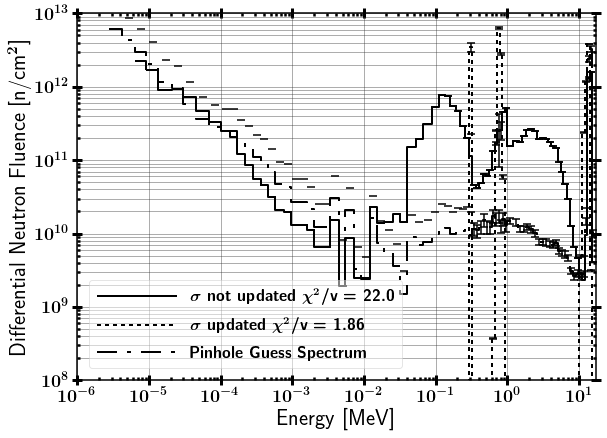
\includegraphics[width=\linewidth]{Figures/Pin3.png}
	\caption{Unfolded Spectrum for pinhole starting with NIF and flat guess.}
	\label{fig:pin}
	\vskip 0.9cm
	\includegraphics[width=\linewidth]{Figures/Bask3.png}
	\caption{Unfolded Spectrum for the basket starting with NIF and flat guess.}
	\label{fig:bask}
	\vskip 0.9cm
	\includegraphics[width=\linewidth]{Figures/KBAS3.png}
	\caption{Unfolded Spectrum for the kinematic base starting with NIF and flat guess.}
	\label{fig:kbas}
\end{figure}

\section{Results}

% I didn't do a ton here since there are some unanswered questions and it seems the results may change.  As of now, these are highly suspect, so it would be interesting to see when using the guess spectrum from a simualtion.  That guess spectrum should be added to the plots.	

A summary of the $\chi^{2}$ statistic and associated p-values are provided in Table \ref{Table:STAY}. The unfolded differential fluence results from STAYSL for the pinhole, basket, and kinematic base are shown in Figures \ref{fig:pin} - \ref{fig:kbas} with the guess spectrum included. The pinhole and basket only include the results without updating the uncertainty which are the minimum $\chi^{2}$ values. 

\begin{table}[h]
	\caption{Summary of unfolded results for pinhole, basket, and kinematic base.}
	\label{Table:STAY}	
	\centering
	\begin{tabular}{|c|c|c|c|}
		\hline
		Location & $\chi^{2}$ / $\nu$ & $\nu$ & p-value \\ \hline
		Pinhole updated uncertainty & 22 & 4 & 0.0 \\ \hline
		Pinhole no updated uncertainty & 1.86 & 4 & 0.11 \\ \hline
		Basket updated uncertainty & 89 & 5 & 0.0 \\ \hline
		Basket no updated uncertainty & 9.5 & 5 & 0.0 \\ \hline
		Kinematic updated uncertainty & 0.71 & 5 & 0.62 \\ \hline
		Kinematic Base no updated uncertainty & 0.48 & 5 & 0.79 \\ \hline
	\end{tabular}
\end{table}

\ Each location is be discussed in further; however, there are some overarching traits to each of the results. First, for the pinhole and basket, the guess spectrum is not particularly well matching to the iterative STAYSL results with or without updating uncertainty. Second, the results in each case provide a better chi-square statistic perform better when the uncertainty is not updated. Not updating the uncertainty allows STAYSL to iterate to a solution that is more consistent with the activation results; however, less and less of the original spectrum is taken into account. Lastly, the 14 MeV source neutrons at the 10.75 keV temperature are attenuated as the neutrons travel farther through the snout which is expected. The total number of neutrons in the source peak energy bin is approximately as expected based on scattering and attenuation. 

\ The pinhole result can only be not rejected for the case where the uncertainty is not updated throughout the iterative process. The p-values associated with the pinhole reject the distribution with updating the uncertainty. Still, there is only a 11\% probability of arriving at such a high chi-square statistic if the pinhole distribution were in fact the energy spectrum of neutrons that created the activations. The solution with uncertainty updates provides a more physical continuous spectrum; however, the chi-square statistic makes the result unusable. The solution without updating uncertainty creates a peak at approximately 800 keV appears in both spectra which is consistent with a compound reaction evaporation spectrum; however, the source of this phenomenon cannot be confirmed. Additionally, A peak at 290 keV is present in the pinhole unfolded results without updating uncertainty. The solution set indicates that the expected neutron fluence is not well modeled at the pinhole. 

\ The basket results are similar to the pinhole with some minor differences. The p-value is zero in both cases which rejects both results; however, some potentially useful information can be obtained as to where the iteration. The spectrum is more spread out for the results with updated uncertainty and not as thermalized as the pinhole which is non physical. The neutrons should be at lower energies further into the snout. Second for the results without updating uncertainty, the 800 keV peak is still present, but the 290 keV is removed. Still, a solution within that has an non-rejectable p-value was not obtained which again indicates that the expected neutron fluence is not well modeled at the basket. 

\ Finally, the results for the kinematic base provided similar fluences with acceptable p-values. The p-value for the updating uncertainty and not updating uncertainty methods are well outside the rejection region. The unfolded kinematic base spectra overlap except from .3 to 4 MeV and match much more closely to the modeled spectra. There is a buildup of fluence in the fast region from the main source term. Additionally, the thermal tail matches the matches the model given the large error expected. Finally, there is large variance in the fluence in the epithermal region, which is an artifact of the foil set. More foils or reactions included would have been able to aid this result. 

\section{Conclusions}

\ Characterizing the neutron energy spectrum in the snout experiment at the NIF through a foil activation experiment provided mixed results. The foil activities and underlying nuclear data were applied in STAYSL to unfold the spectrum with STAYSL for the pinhole, basket, and kinematic base locations in the snout. The results where the uncertainty was updated show general attenuation of the DT source to lower energy regions. The results where the uncertainty was not updated each iteration produced spectra that more closely matched the activation products; however, these results are less physical. 

\ The unfolded neutron spectra for the pinhole and kinematic base arrived at acceptable p-values for at least one method. A non-rejected solution was not accomplished for the basket. Three possible reasons for the discrepancies include the foil material parameters, modeled spectra, and uncertainty in the NIF source.  The unfolded neutron spectrum results reinforce the necessity of having a well modeled initial guess spectrum for the generalized least-squares minimization. 

	\ifCLASSOPTIONcaptionsoff
	\newpage
	\fi
	
	\begin{thebibliography}{17}
		% 1 
		\bibitem{Knoll} 
		G. F. Knoll, Radiation Detection and Measurement, Ann Arbor,
		Michigan: Wiley, 2010.
		\bibitem{NETF}
		“AF NETF Graphite Standard Pile”, WADD-TR-61-174, Air Force Systems Command (1962).
		\bibitem{Will}
		W. Johnston, “Characterizing the Neutron Energy Distribution of the AFIT Building 470 Graphite Pile,” NENG 725, 2018.
		\bibitem{Bevins}
		J. E. Bevins, “Calibration of AFIT Graphite Pile to Account for 241Am Ingrowth in the 239PuBe13 Source,” Air Force Institute of Technology, Wright-Patterson Air Force Base, OH, 2009. 
		\bibitem{Bogetic}
		S. Bogetic, “Passive 18x Snout on TANDM 90-348,” University of California - Berkeley, 2018.  
		\bibitem{STAYSL}
		B. Rearden, M. Jessee, and Eds., User Guide for the STAYSL PNNL Suite of
		Software Tools, PNNL-22253, Pacic Northwest National Laboratory, Richland,
		WA, February 2013.
		\bibitem{Me}
		N. J. Quartemont, "NIF ETA," August 2018. [Online]. Available:
		https://github.com/nickquartemont/NENG612
		\bibitem{Luciano2012a}
		N. P. Luciano, “A High-Energy Neutron Flux Spectra Measurement Method for
		the Spallation Neutron Source,” Master's thesis, University of Tenessee Knoxville,
		2012.
		\bibitem{MCNP}
		MCNP6 Users Manual - Code Version 6.1, LA-CP-13-00634 (May 2013)
		\bibitem{NIFSrc}
		C. B. Yeamans and B. E. Blue, "National Ignition Facility Neutron 
		Sources," in HEART, Tuscon, 2018. 
		\bibitem{Appelbe}
		B. Appelbe and J. Chittenden, "Relativistically Correct DD and DT 
		Neutron Spectra,," High Energy Density Phys., vol. 11, no. 1, pp. 
		30-35, 2014.
		\bibitem{Kuijpers1977}
		L. Kuijpers, R. Herzing, P. Cloth, D. Filges, and R. Hecker, “On the Determination of Fast Neutron Spectra with Activation 
		Techniques; its Application in a Fusion Reactor Blanket Model,” Nuclear Instruments and Methods, vol. 144, no. 2, pp. 215-224, 1977. 
		\bibitem{Vagena2018b}
		E. Vagena, K. Theodorou, and S. Stoulos, “Thick-foils Activation Technique
		for Neutron Spectrum Unfolding with the MINUIT Routine: Comparison
		with GEANT4 simulations," Nuclear Instruments and Methods in Physics
		Research, Section A: Accelerators, Spectrometers, Detectors and Associated
		Equipment, vol. 887, no. January, pp. 64-69, 2018.
%		\bibitem{Leo}
%		W. R. Leo, Techniques for Nuclear and Particle Physics Experiments, New York: Springer-Verlag, 1994. 
		\bibitem{Reginatto2010}
		M. Reginatto, “Overview of Spectral Unfolding Techniques and Uncertainty Esti-
		mation,” Radiation Measurements, vol. 45, no. 10, pp. 1323-1329, 2010.
		\bibitem{Perey1977}
		F. G. Perey, “Least-Squares Dosimetry Unfolding: The Program STAY'SL
		(ORNL/TM-6062),” Oak Ridge, Tennessee, 1977.
		\bibitem{Greenwood2016}
		L. Greenwood and C. Johnson, “Least-Squares Neutron Spectral Adjustment with
		STAYSL PNNL," EPJ Web of Conferences," vol. 106, p. 07001, 2016.
		\bibitem{PeakEZ}
		B. Rooney, S. Garner, P. Felsher, and P. Karpius, “PeakEasy Version 4.97.” [Computer Program] Los Alamos National Laboratory, 2018.
		\bibitem{Iter}
		J. E. Bevins, STAYSL.py," 2018. [Online]. Available: https://github.com/jamesbevins/PyScripts/tree/master/src/Unfolding.
	\end{thebibliography}
	
\end{document}


